\documentclass{main.tex}[subfiles]
\begin{document}
\newpage
\section{Задача распознавания символов Брайля}
\subsection{Общая постановка задачи и особенности рельефно-то\-чеч\-но\-го шрифта}
В рельефной азбуке, разработанный Луи Брайлем в 1824 году, каждая буква обозначается последовательностью выпуклых точек, расположенных в ячейке $ 3 \times 2 $ точки. Ячейки располагаются в строку справа налево, как привычные нам буквы (рис. \ref{fig:brl_example:written}).
Каждая точка может быть выдавлена или пропущена, т. о. всего возможны лишь $2^{3\cdot2}=64$ комбинации; поэтому некоторые символы (цифры, нотные знаки и т. д.) записываются двумя, тремя или даже четырьмя знаками.
Все буквы латинского и кириллического алфавита требуют для записи только одной клетки, но в английском языке разработана система сокращений (contractions) -- например, для экономии места слово "across"\hspace{0pt} можно писать как "acr"\hspace{0pt}, т. к. по плотности расположения знаков на странице брайлевский шрифт значительно уступает привычному нам способу записи.
Тексты, написанные с использованием сокращений, называются <<Брайль уровня 2>> ("Grade 2 Braille").
В русском языке система сокращений практически не используется и в стандартах не описана.

\begin{figure}[h]
    \centering
    \begin{subfigure}{.5\textwidth}
        \centering
        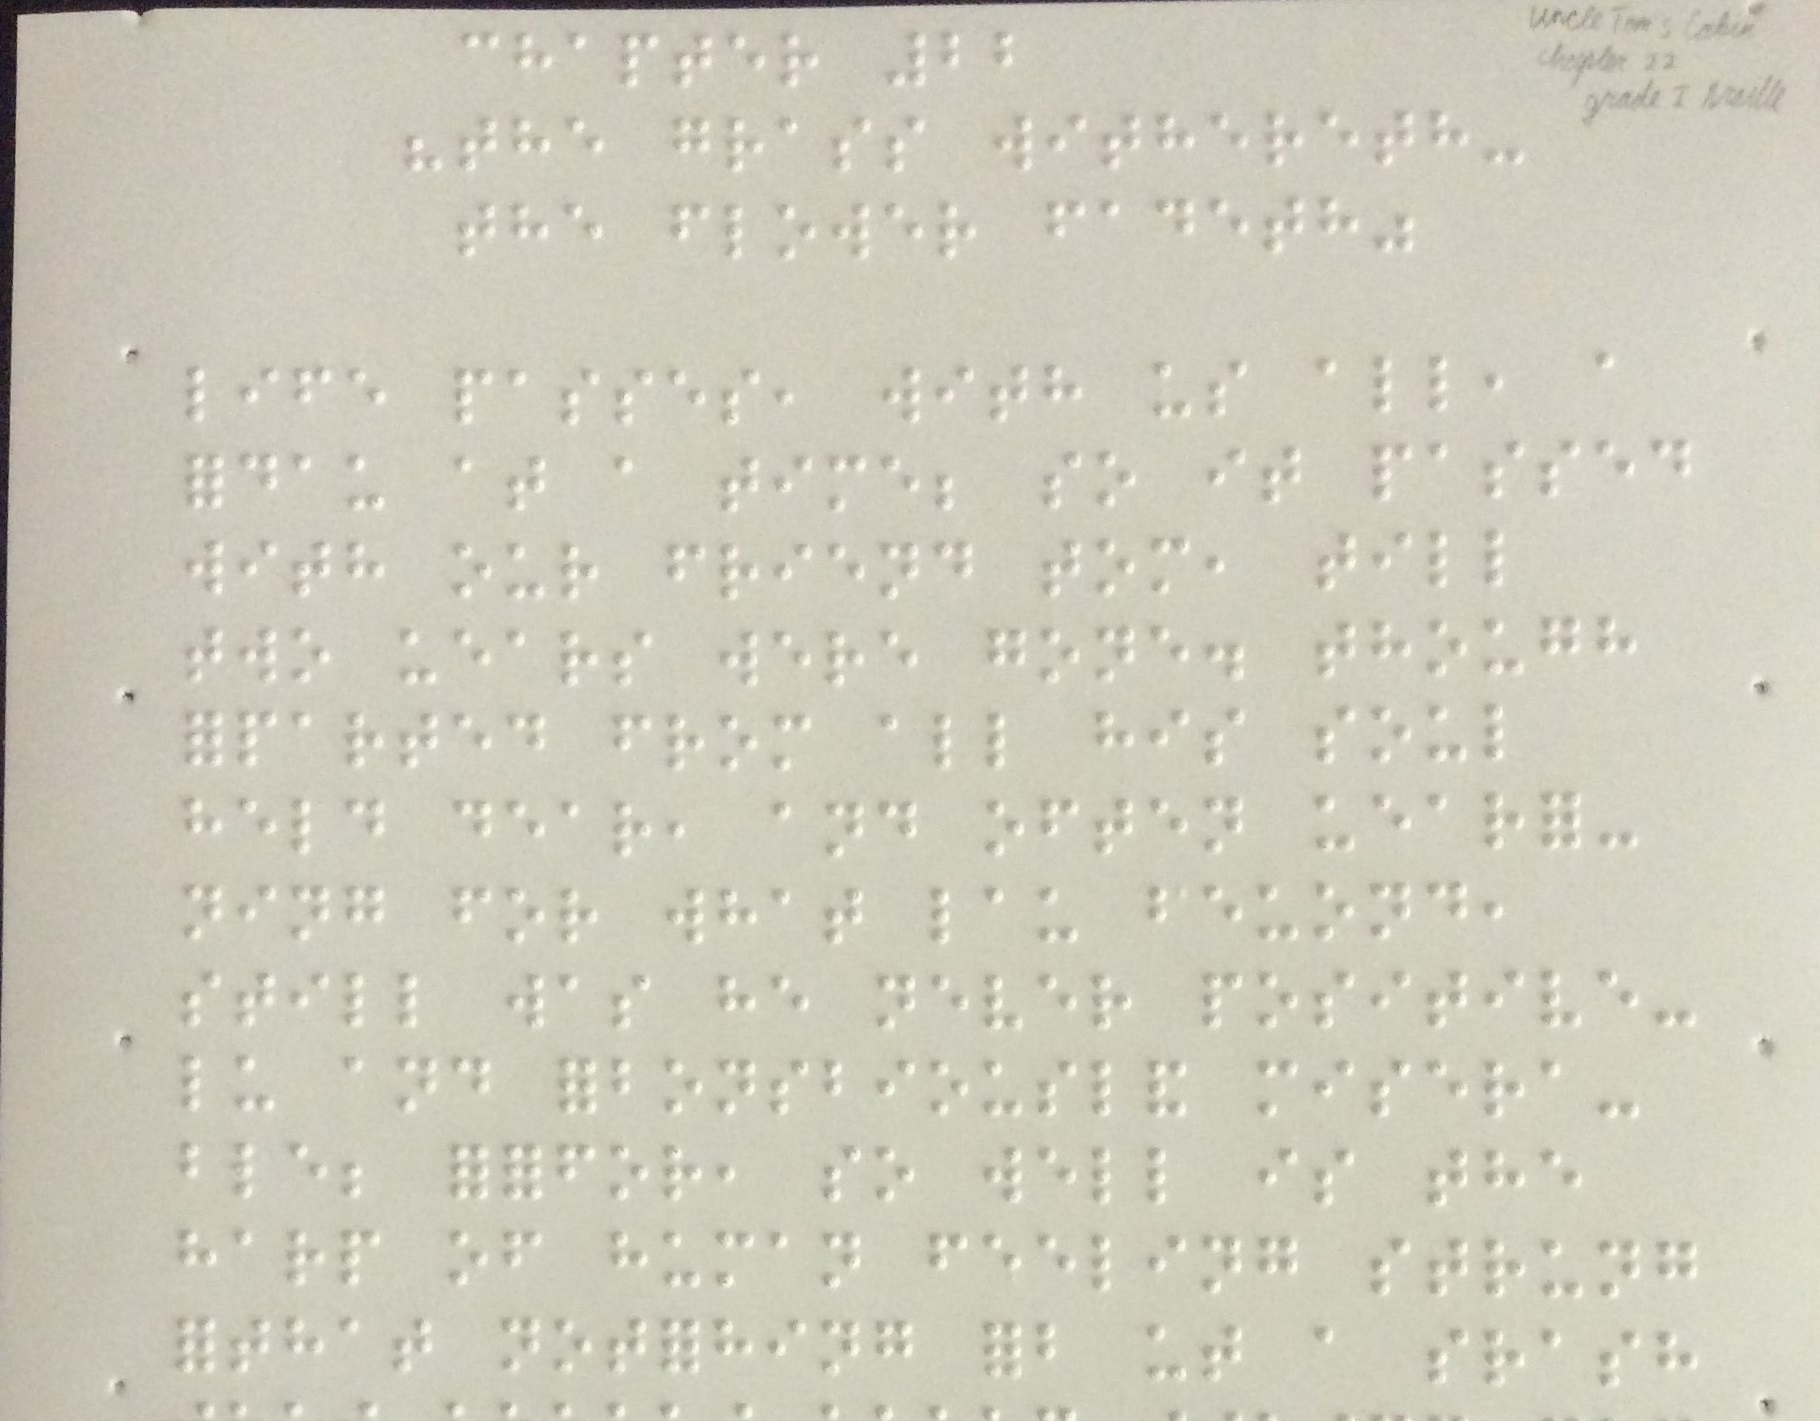
\includegraphics[width=.9\myPictWidth]{brl_writing_uncle_tom}
        \caption{рукопись}
        \label{fig:brl_example:written}
    \end{subfigure}%
    \begin{subfigure}{.5\textwidth}
        \centering
        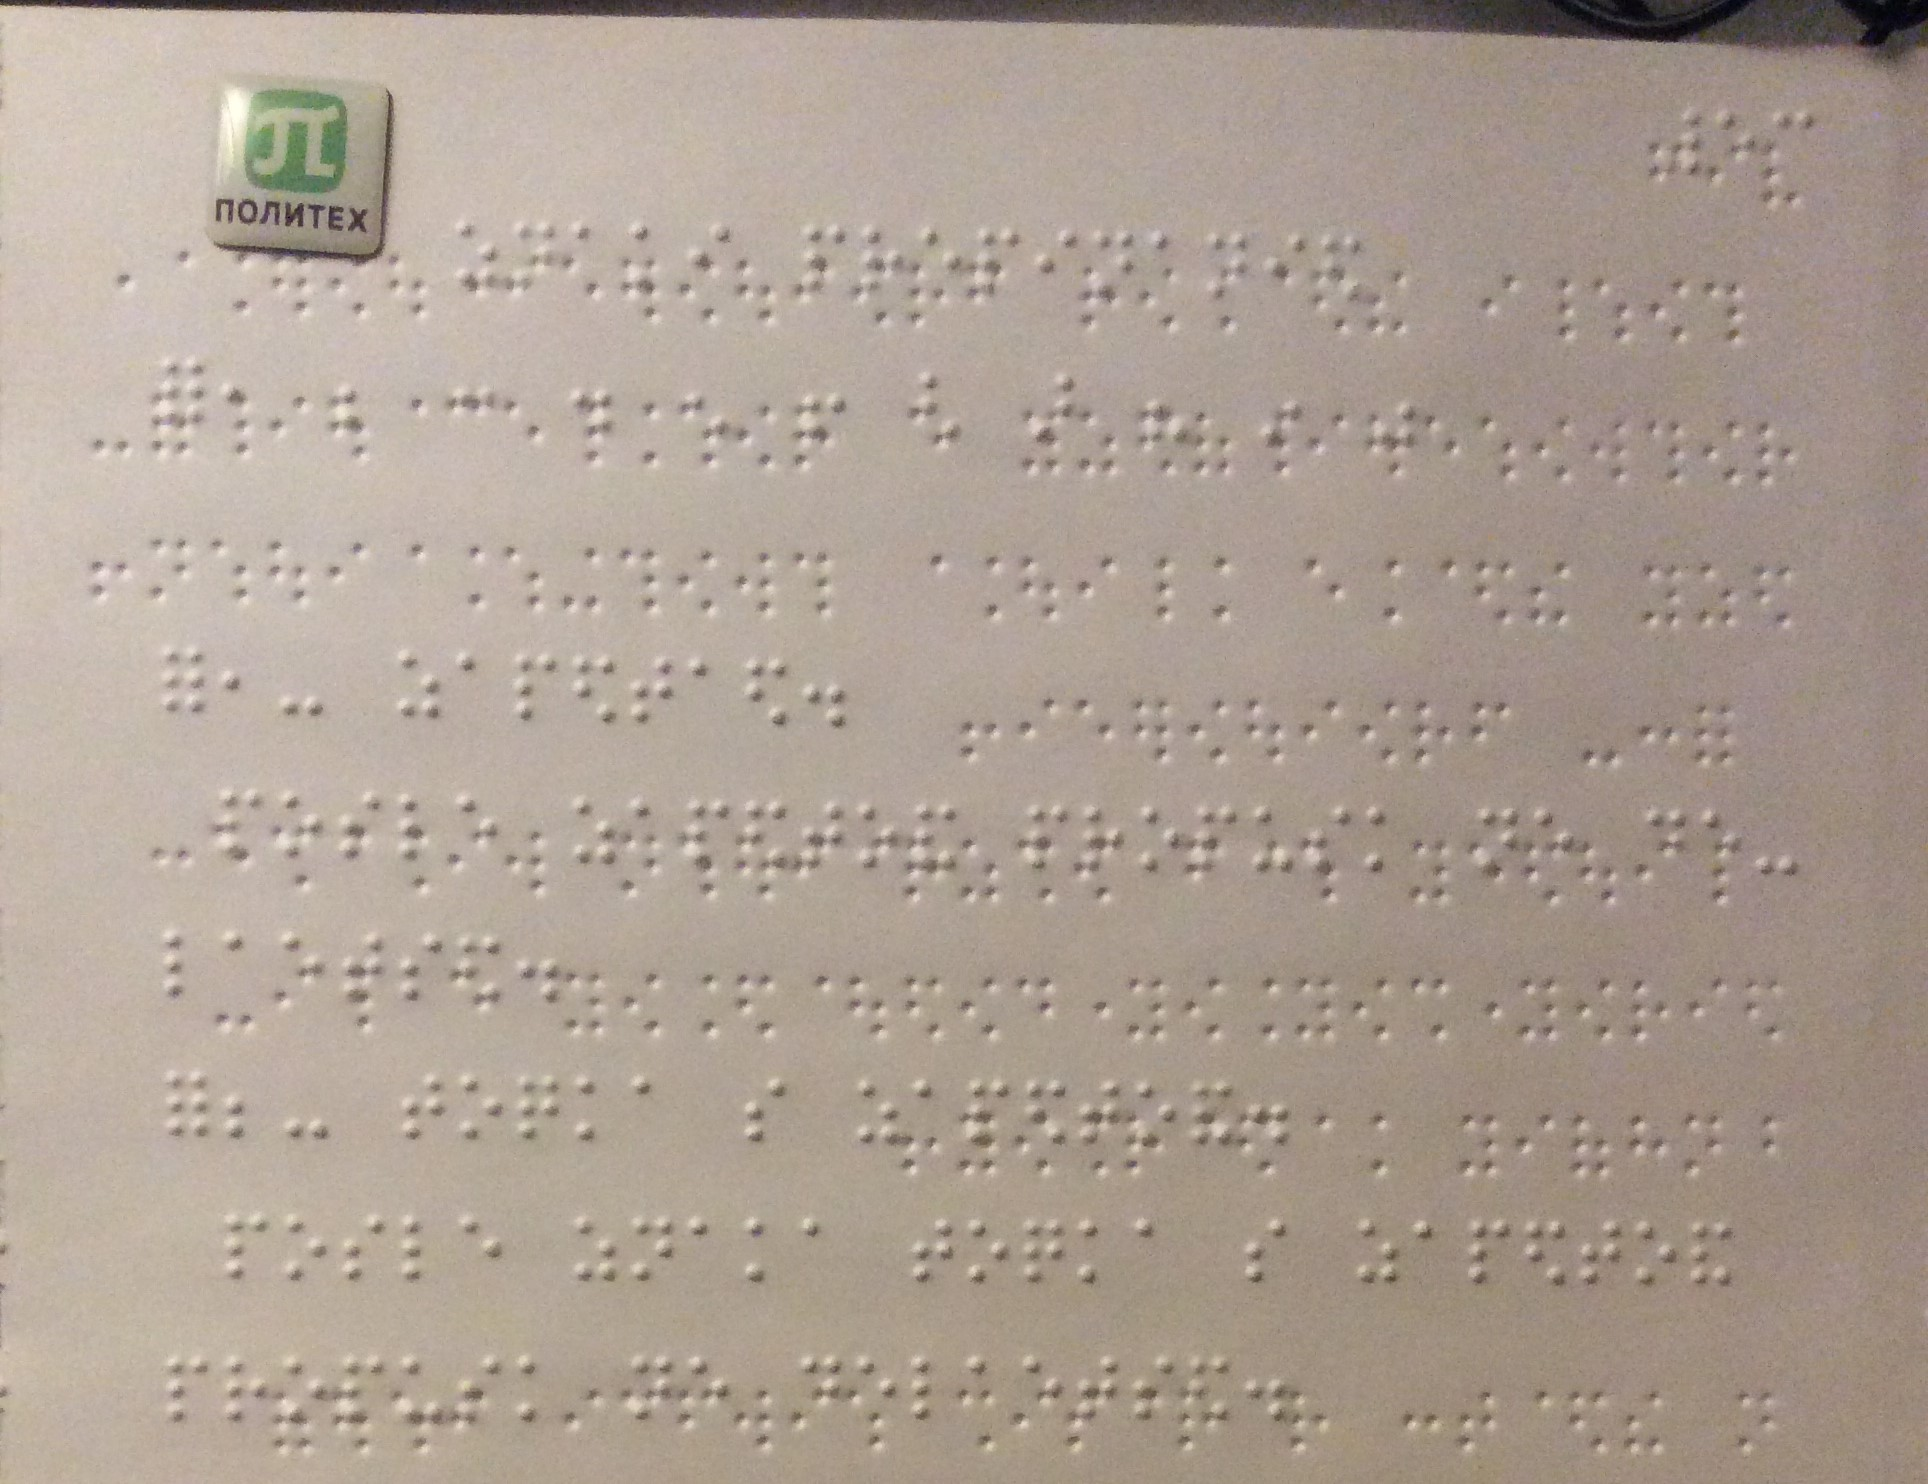
\includegraphics[width=.9\myPictWidth]{brl_book_golubina}
        \caption{книга}
        \label{fig:brl_example:book}
    \end{subfigure}
    \caption{Листы с рельефно-точечным шрифтом Брайля}
    \label{fig:brl_example}
\end{figure}

При письме точки выкалываются металлическим грифелем через трафарет; используется только одна сторона листа.
Также издаются книги, где используются обе стороны (рис. \ref{fig:brl_example:book}).

Задача заключается в следующем: на вход программе поступает фотография рукописного или книжного листа, снятая на камеру фотоаппарата или смартфона (рис. \ref{fig:brl_example}); требуется найти и распознать символы шрифта Брайля, определить их порядок и выдать ответ в виде последовательности строк.
Формально в задачу не входит перевод шеститочечных символов в обычные (для этого существует особое ПО, например, Liblouis\footnote{\href{http://liblouis.org/}{liblouis.org}}), но зачастую это удобно сделать, чтобы оценить количество ошибок распознавания.

Все буквы имеют одинаковый размер, точки расположены в определённых местах и на определённом расстоянии друг от друга, что упрощает задачу распознавания.
Тем не менее, появляются дополнительные сложности по сравнению с задачей распознавания обычных символов:

\begin{enumerate}[noitemsep]
    \item Точки не выделены цветом, только рельефом.
    Следовательно, при распознавании по фотографии программа ориентируется на отбрасываемые тени.
    Как было отмечено ранее, в книгах текст печатается на обеих сторонах, и углубления (точки на обороте) на фотографиях даже эксперт может перепутать с точками на лицевой стороне.
    Поэтому, как правило, к исходным данным предъявляется следующее требование: свет всегда должен падать в определённом направлении (например, строго спереди и сверху или строго сзади и сверху от фотографируемой поверхности).
    \item Однотипность точек в азбуке Брайля усложняет классификацию букв и определение их границ.
    Например, при нахождении символа, составленного из трёх точек, расположенных в одном столбце, сложно понять, это точки первого столбца или второго; две точки одна под другой могут быть точками из одной клетки или из двух клеток в разных строках.
    Поэтому чаще всего детекторы работают в два этапа:
    \begin{enumerate}[noitemsep]
        \item Поиск строк на фотографии
        \item Поиск и классификация отдельных символов в строках.
    \end{enumerate}
\end{enumerate}

\subsection{Обзор существующих решений}
% TODO write a bit about SSL, maybe cite some articles (? at least IOvo's)
\subsubsection{Подходы к распознаванию}
Программы распознавания шрифта Брайля разрабатываются начиная с конца XIX века.
В первую очередь они предназначены для брайлевских сканеров, при использовании которых строки на фотографии находятся на параллельных прямых.
Как правило, такие программы работают по следующей схеме:
\begin{enumerate}[noitemsep]
    \item Предобработка изображения (например, фильтрация шумов, повышение контрастности)
    \item Поиск отдельных точек (например, с помощью преобразования Хоу или метода опорных векторов)
    \item Восстановление воображаемых линий, на которых расположены точки.
\end{enumerate}
Некоторые алгоритмы после восстановления линий выполняют поиск точек ещё раз (уточнение точек).
Подробные обзоры различных методик даны в статьях \cite{isayed2015review, shokat2020review}.

Прогресс последних лет в области машинного обучения, в особенности появление свёрточных нейронных сетей, сделали возможным создание программ, надёжно распознающих тексты на изображениях, которые сняты в неидеальных условиях.
Например, в 2020 году опубликована статья, авторы которой выполняют поиск брайлевских строк с помощью Faseter R-CNN, после чего ещё одна нейросеть выполняет поиск отдельных символов \cite{baumgartner2020app}.
Реализованная в этой работе программа была оформлена в виде Android-приложения, которое может распознавать тексты по фотографиям, снятым на камеру смартфона, при условии, что лист ровный и освещён яркой лампой, которую нужно разместить внизу страницы.
В другой разработке свёрточная нейронная сеть используется не на этапе поиска линий, а только при классификации символов \cite{alsalman2021}.
Но надо отметить, что эти две программы, во-первых, работают только с односторонними документами, и, во-вторых, пригодны лишь в случае, когда сфотографированный лист не изогнут, поскольку предполагается, что строки лежат на параллельных прямых линиях.

Особый интерес представляют алгоритмы, основанные на нейронных сетях UNet \cite{li2020braunet} и RetinaNet \cite{ovodov2020, ovodov2021}.
В них предлагается вместо поиска строк или точек находить на изображении шеститочечные брайлевские символы, которые затем складываются в строки.
Это позволяет успешно обрабатывать даже те фотографии, где лист изогнут или помят.
Исходный код программы AngelinaReader, созданной автором \cite{ovodov2020, ovodov2021}, находится в открытом доступе\footnote{\href{https://github.com/IlyaOvodov/AngelinaReader}{github.com/IlyaOvodov/AngelinaReader}}.

В статье \cite{ortoncelli2021} также описывается способ постобработки распознанных текстов, который позволяет уменьшить число ошибок распознавания.

\subsubsection{Наборы данных}\label{section:datas}

До недавнего времени в свободном доступе не было размеченных фотографий текта, написанного шрифтом Брайля.
В 2018 году был опубликован набор DSBI (DataSet of Braille Images) \cite{li2018dsbi}, содержащий 114 аннотированных сканов; текст нанесён с двух сторон и аннотации к каждой фотографии приведены как для точек на лицевой стороне, так и для точек на обороте.

Позже разработчик программы Angelina Reader опубликовал набор An\-ge\-li\-na\-Da\-ta\-set \footnote{\href{https://github.com/IlyaOvodov/AngelinaDataset}{github.com/IlyaOvodov/AngelinaDataset}}, содержащий 240 размеченных фотографий брайлевского текста (212 двусторонних страниц из книг и 28 рукописных).
Фотографии, включённые в AngelinaDataset, были сняты в следующих условиях:
\begin{enumerate}[noitemsep]
	\item Лист расположен горизонтально и сфотографирован сверху
	\item Свет падает спереди от фотографирующего, т. е. сверху по отношению к фотографируемому листу.
\end{enumerate}

Некоторые исследователи используют частично или полностью сгенерированную выборку \cite{baumgartner2020app, ortoncelli2021}.

\subsection{Цели и задачи настоящей работы}

Несмотря на значительный прогресс в разработке программ детектирования брайлевского текста, остаётся ряд нерешённых проблем.
Программа Angelina Braille Reader, которая показывает наилучшие результаты среди тех, которые представлены в работах \cite{li2018dsbi, li2020braunet, ovodov2020} при обучении на наборе DSBI (т. е. самое высокое значение F1-меры при запуске на валидационной части -- $0.9981$), всё же иногда допускает ошибки даже при распознавании фотографий, снятых в требуемых условиях (см. рис. \ref{fig:recogn_mistakes} в приложении).

Данная работа направлена на улучшение качества работы алгоритмов распознавания шрифта Брайля путём применения полуконтролируемого обучения на примере программы Angelina Braille Reader. % TODO find better words to describe goals; ? write what is F1 here? What is SSL? Why the idea of SSL came to me (small dataset size, some symbols not present in current datasets)?
Поставлены следующие задачи:
\begin{enumerate}
	\item Собрать выборку из неразмеченных фотографий двустороннего брайлевского текста, объём которой кратно превосходит объём An\-ge\-li\-na\-Da\-ta\-set и DSBI. Изображения должны быть получены с соблюдением требований, указанных в разделе \ref{section:datas}.
	Получить псевдометки с помощью нейронной сети, обученной на An\-ge\-li\-na\-Da\-ta\-set  и DSBI.
	\item  Разработать и реализовать алгоритм улучшения меток, основанный на семантике (структуре слов и предложений в распознанном тексте).
	Применить его к автоматически размеченным данным, полученным на предыдущем этапе.
	\item Обучить нейронную сеть на объединённом наборе: DSBI + An\-ge\-li\-na\-Da\-ta\-set + данные с улучшенными псевдометками.
	Сравнить показатели качества этой нейронной сети и обученной только на DSBI + An\-ge\-li\-na\-Da\-ta\-set при запуске на валидационной части DSBI, An\-ge\-li\-na\-Da\-ta\-set и данных с псевдометками.
\end{enumerate}

\end{document}
